%%
%% $Id$
%%
%% Copyright (c) 2007-2008 Christian Fehler
%% Copyright (c) 2007-2008 Benjamin Mies
%%


\chapter{Perspektive}\label{Perspective}

In diesem Kapitel werden die Zukunftspersektiven für das \gtitool besprochen.
Bei der Implementierung wurde besonderer Wert darauf gelegt, dass das \gtitool
leicht zu erweitern sein muss. Der dadurch entstandene Aufwand konnte dadurch
gerechtfertigt werden, dass Erweiterungen in der Zukunft leichter und somit
schneller integriert werden können.


\section{Graphische Komponenten implementieren}\label{PerspectiveGraphics}

Wie in Abschnitt \ref{Graph} beschrieben verwenden wir zur graphischen
Darstellung der Automaten die Bibliothek JGraph. Diese Bibliothek bietet einen
sehr großen Funktionsumfang, der von uns nicht komplett ausgeschöpft werden
musste. Eine mögliche Implementierung für die Zukunft wäre es, diese Bibliothek
durch eine eigene Implementierung zu ersetzen, die dann nur den gewünschten
Umfang bietet und somit leichter zu warten und zu erweitern ist.\vspace{10pt}

Da eine solche Implementierung sehr viel Zeit in Anspruch nehmen würde, war es
uns im Rahmen der Diplomarbeit nicht möglich, neben den umgesetzten Komponenten
auch noch die graphischen Komponenten selbst zu implementieren. JGraph bot uns
die Möglichkeit sehr schnell und einfach bereits brauchbare Ergebnisse zu
erzielen. Es mussten einige in \ref{GraphJGraphAdaptation} beschriebene
Anpassungen vorgenommen werden, damit das Ergebnis unseren Vorstellungen
entsprach, aber diese waren im Gegensatz zu einer vollständigen Implementieren
zeitlich nicht so komplex.\vspace{10pt}

Zu einer möglichen Umsetzung ist zu sagen, dass sowohl Zustände wie auch
Übergänge modiliert werden müssen. Was gerade bei der Verwendung von parallel
Übergängen ein größeres Problem sein könnte, da dort die Übergänge nicht auf
einer Linie verlaufen. Der größte Nutzer bei einer eigenständigen
Implementierung wäre, das Änderungen leichter eingepflegt werden könnten, da
dies bei der sehr komplexen Implementierung von JGraph meistens problematisch
war.


\section{Reguläre Ausdrücke}

Die wohl wichtigste und komplexeste Erweiterung die für die Zukunft geplant
ist, ist die Unterstützung von regulären Ausdrücken. Der Benutzer soll somit in
der Lage sein, einen regulären Ausruck wie
(\Symbol{a}$\mid$\Symbol{b})*\Symbol{a}\Symbol{b}\Symbol{b} eingeben zu können.
Anschließend sollen im Idealfall mehrere Möglichkeiten bestehen, mit diesem
Ausdruck weiter zu arbeiten. Diese Möglichkeiten sollen nun kurz angesprochen
werden.\vspace{10pt}

Der eingegebene reguläre Ausdruck soll mit dem in \gticitepage{Compilers}{159ff}
beschriebenen McNaughton-Yamada-Thompson Algorithmus in einen Automaten
umgewandelt werden können. Diese Umwandlung sollte, wie die anderen
Umwandlungen auch, schrittweise durchgeführt werden. Dadurch soll es dem
Benutzer ermöglicht werden, den zur Umwandlung benutzten Algorithmus besser zu
verstehen. Abbildung \ref{FigureThompson} zeigt das Ergebnis, das bei einer
solchen Umwandlung entstehen würde.\vspace{10pt}

\begin{figure}[h!]
\begin{center}
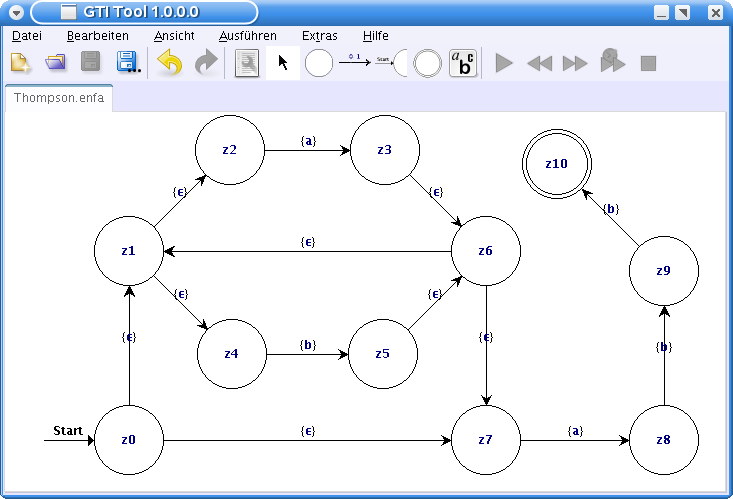
\includegraphics[width=12cm]{../images/thompson.png}
\caption{McNaughton-Yamada-Thompson Algorithmus}
\label{FigureThompson}
\end{center}
\end{figure}

Eine weitere Verwendungsmöglichkeit eines regulären Ausdruck wäre das direkte
Umwandeln in einen DEA. Dieser Algorithmus wird in
\gticitepage{Compilers}{175ff} beschrieben und verwendet die Funktionen
\textit{nullable}, \textit{firstpos}, \textit{lastpos} und \textit{followpos},
um die Umwandlung durchzuführen. Bei der Umsetzung müsste das Berechnen dieser
Funktionen in irgendeiner Weise dargestellt werden, idealerweise anhand des
Syntaxbaumes des regulären Ausdrucks. Ein mögliches Ergebnis der direkten
Umwandlung ist in Abbildung \ref{FigureRegExDFA} zu sehen.

\begin{figure}[h!]
\begin{center}
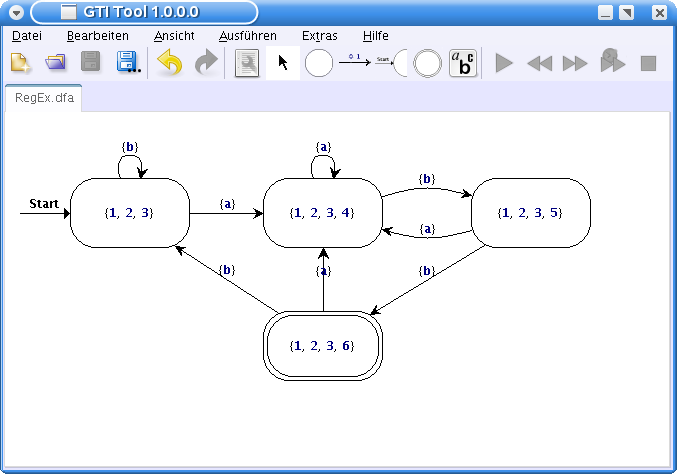
\includegraphics[width=12cm]{../images/regex_dfa.png}
\caption{Direkte Umwandlung in einen DEA}
\label{FigureRegExDFA}
\end{center}
\end{figure}


\section{\LaTeX-Export}

TODOCF


\section{Grammatik Erweiterungen}

TODOBM: Linksrekursion, Linksrefaktorisierung, Wort direkt eingeben können


\section{Erkannte Wörter ausgeben}

TODOCF


\section{Eingabe von mehreren Wörtern}

TODOCF


\section{Benutzerinteraktion erhöhen}

TODOCF


\section{Auto-Layout}\label{PerspectiveAutoLayout}

TODOBM
